\UseRawInputEncoding
%=============================================================================
% search-o-SAURS Report -- Boolean Information Retrieval System
% Cranfield Aeronautics Corpus
%=============================================================================
\documentclass[12pt,a4paper]{article}

%--- Packages ---------------------------------------------------------------
\usepackage[margin=1in]{geometry}
\usepackage{graphicx}
\usepackage{xcolor}
\usepackage{booktabs}
\usepackage{array}
\usepackage{longtable}
\usepackage{listings}
\usepackage[colorlinks=true,linkcolor=blue,urlcolor=blue,citecolor=blue]{hyperref}
\usepackage{amsmath}
\usepackage{amssymb}
\usepackage{tikz}
\usetikzlibrary{shapes.geometric, arrows.meta, positioning}
\usepackage{float}
\usepackage{caption}
\usepackage{fancyhdr}
\usepackage{enumitem}

%--- Page style -------------------------------------------------------------
\pagestyle{fancy}
\fancyhf{}
\fancyhead[L]{\small search-o-SAURS}
\fancyhead[R]{\small Programming Assignment~I}
\fancyfoot[C]{\thepage}
\renewcommand{\headrulewidth}{0.4pt}

%--- Listings style ---------------------------------------------------------
\definecolor{codebg}{RGB}{245,245,245}
\definecolor{codegreen}{RGB}{0,128,0}
\definecolor{codegray}{RGB}{128,128,128}
\definecolor{codeblue}{RGB}{0,0,180}

\lstdefinestyle{pythonstyle}{
    backgroundcolor=\color{codebg},
    basicstyle=\ttfamily\footnotesize,
    keywordstyle=\color{codeblue}\bfseries,
    stringstyle=\color{codegreen},
    commentstyle=\color{codegray}\itshape,
    numberstyle=\tiny\color{codegray},
    numbers=left, numbersep=5pt,
    frame=single, breaklines=true, showstringspaces=false,
    tabsize=4, captionpos=b, language=Python,
    morekeywords={self,True,False,None},
}
\lstdefinestyle{shellstyle}{
    backgroundcolor=\color{codebg},
    basicstyle=\ttfamily\footnotesize,
    frame=single, breaklines=true, showstringspaces=false,
    captionpos=b, language=bash,
}
\lstdefinestyle{outputstyle}{
    backgroundcolor=\color{codebg},
    basicstyle=\ttfamily\scriptsize,
    frame=single, breaklines=true, showstringspaces=false,
    captionpos=b, numbers=none,
}
\lstset{style=pythonstyle}

%=============================================================================
\begin{document}

%=============================================================================
% COVER PAGE
%=============================================================================
\begin{titlepage}
\centering
\vspace*{2cm}
{\LARGE\bfseries Information Retrieval}\\[0.4cm]
{\Large\bfseries Programming Assignment~I}\\[2cm]
{\huge\bfseries A Boolean Information Retrieval System\\for the Cranfield Aeronautics Corpus}\\[2cm]
{\Large\bfseries Group: search-o-SAURS}\\[1.5cm]
\begin{tabular}{l l}
\toprule
\textbf{Name} & \textbf{Roll Number} \\
\midrule
Utsa Ghosh & 23CS10090 \\
Antariksh Das & 23CS10086 \\
Raktim Kundu & 23CS30044 \\
Souhardya Dandapat & 23CS30054 \\
Sharanya Baidya & 23CS30064 \\
\bottomrule
\end{tabular}
\vfill
\end{titlepage}

%=============================================================================
\tableofcontents
\newpage

%=============================================================================
\section{Introduction}
\label{sec:introduction}
%=============================================================================

This report describes \textbf{search-o-SAURS}, a Boolean Information Retrieval
system built for Programming Assignment~1.  The system processes the
\textbf{Cranfield~1400} collection (1,400 aeronautics research abstracts) and
supports \textbf{AND/OR} Boolean queries over a constructed inverted index.

The end-to-end transformation is:
\begin{center}
\textit{Raw Corpus}
$\;\to\;$ \textit{Preprocessing}
$\;\to\;$ \textit{Inverted Index}
$\;\to\;$ \textit{Boolean Query}
$\;\to\;$ \textit{Matching Document IDs}
\end{center}

The system is implemented entirely in Python~3 using only standard-library
modules---no external IR libraries---as required by the assignment.

%=============================================================================
\section{Assignment Requirements}
\label{sec:requirements}
%=============================================================================

The assignment requires:
\begin{enumerate}[noitemsep]
  \item \textbf{Preprocessing}: Tokenization, normalization, stemming (Porter), and stop-word removal.
  \item \textbf{Inverted Index}: Map each term to the list of documents containing it.
  \item \textbf{Boolean Retrieval}: Support AND/OR queries over two terms; output matching document IDs.
  \item \textbf{No external IR libraries}; self-contained implementation.
  \item \textbf{Deliverables}: Source code, README, and a methodology report with program listing.
\end{enumerate}

Our implementation satisfies all requirements and additionally provides:
British--American spelling normalization, token deduplication,
file-based binary search on the index, and adaptive AND merging with galloping search.

%=============================================================================
\section{Dataset}
\label{sec:dataset}
%=============================================================================

The Cranfield collection uses field markers: \texttt{.I}~(document~ID),
\texttt{.T}~(title), \texttt{.A}~(author), \texttt{.B}~(bibliographic reference),
\texttt{.W}~(abstract).

\textbf{Design decision}: We process \texttt{.T} and \texttt{.W} fields only
(title + abstract), as these contain the substantive technical content.
Author names and journal references do not contribute to subject-based retrieval.
The stop-word list (\texttt{stopwords.txt}) contains 357 common English words.

%=============================================================================
\section{System Architecture}
\label{sec:architecture}
%=============================================================================

\begin{figure}[H]
\centering
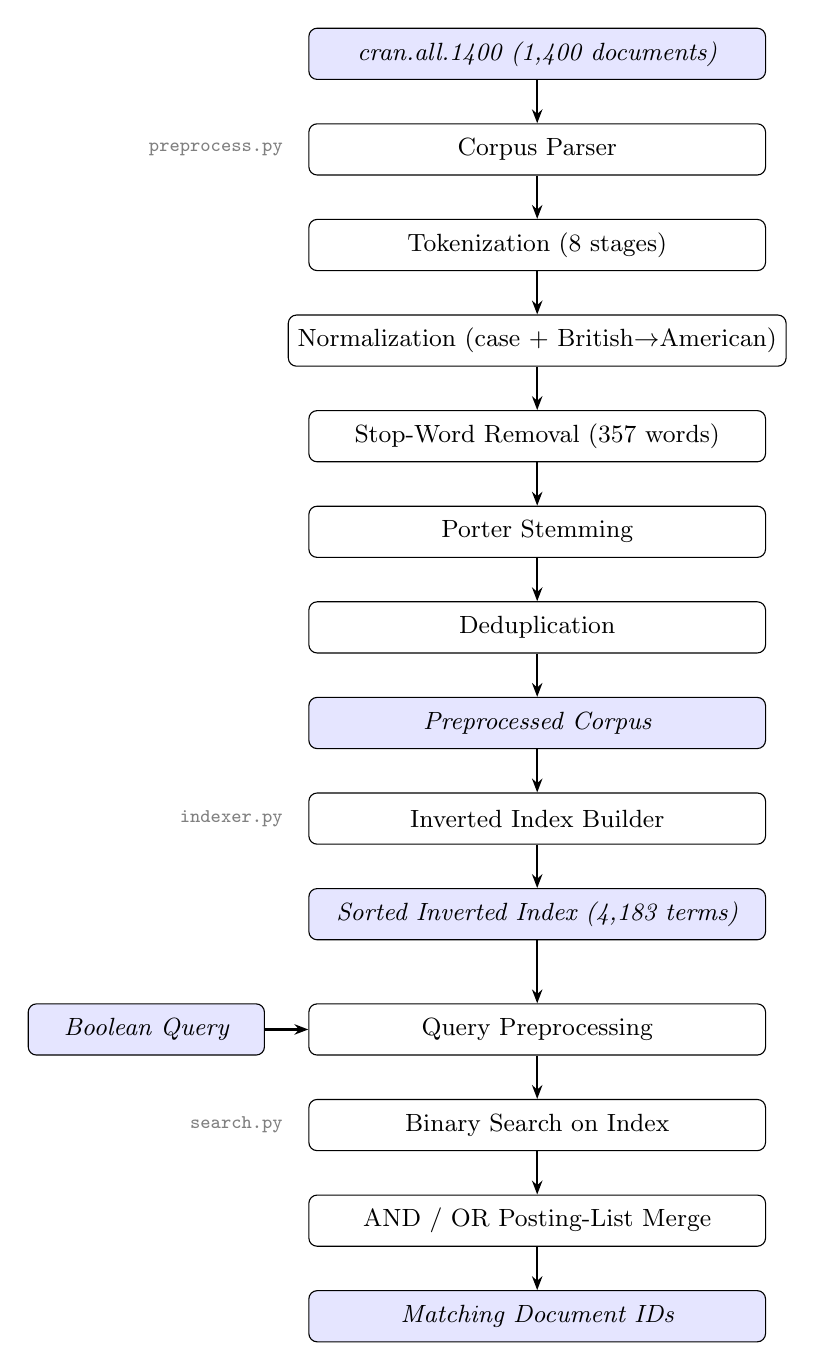
\begin{tikzpicture}[
    node distance=0.55cm,
    box/.style={rectangle, draw, rounded corners=3pt, minimum width=5.8cm,
                minimum height=0.65cm, text centered, font=\small},
    data/.style={rectangle, draw, fill=blue!10, rounded corners=3pt,
                 minimum width=5.8cm, minimum height=0.65cm, text centered,
                 font=\small\itshape},
    arrow/.style={-{Stealth[length=5pt]}, thick},
]
\node[data] (corpus) {cran.all.1400 (1,400 documents)};
\node[box, below=of corpus] (parse) {Corpus Parser};
\node[box, below=of parse] (tokenize) {Tokenization (8 stages)};
\node[box, below=of tokenize] (normalize) {Normalization (case + British$\to$American)};
\node[box, below=of normalize] (stopwords) {Stop-Word Removal (357 words)};
\node[box, below=of stopwords] (stem) {Porter Stemming};
\node[box, below=of stem] (dedup) {Deduplication};
\node[data, below=of dedup] (processed) {Preprocessed Corpus};
\node[box, below=of processed] (indexer) {Inverted Index Builder};
\node[data, below=of indexer] (index) {Sorted Inverted Index (4,183 terms)};
\node[box, below=0.8cm of index] (qpreprocess) {Query Preprocessing};
\node[data, left=of qpreprocess, minimum width=3cm] (query) {Boolean Query};
\node[box, below=of qpreprocess] (bsearch) {Binary Search on Index};
\node[box, below=of bsearch] (merge) {AND / OR Posting-List Merge};
\node[data, below=of merge] (results) {Matching Document IDs};

\draw[arrow] (corpus)--(parse);  \draw[arrow] (parse)--(tokenize);
\draw[arrow] (tokenize)--(normalize); \draw[arrow] (normalize)--(stopwords);
\draw[arrow] (stopwords)--(stem); \draw[arrow] (stem)--(dedup);
\draw[arrow] (dedup)--(processed); \draw[arrow] (processed)--(indexer);
\draw[arrow] (indexer)--(index); \draw[arrow] (index)--(qpreprocess);
\draw[arrow] (query)--(qpreprocess);
\draw[arrow] (qpreprocess)--(bsearch); \draw[arrow] (bsearch)--(merge);
\draw[arrow] (merge)--(results);

\node[left=0.2cm of parse, font=\scriptsize\ttfamily, text=gray]{preprocess.py};
\node[left=0.2cm of indexer, font=\scriptsize\ttfamily, text=gray]{indexer.py};
\node[left=0.2cm of bsearch, font=\scriptsize\ttfamily, text=gray]{search.py};
\end{tikzpicture}
\caption{Complete pipeline architecture.}
\label{fig:arch}
\end{figure}

Three scripts: \texttt{search-o-SAURS\_preprocess.py} (455 lines),
\texttt{search-o-SAURS\_indexer.py} (70 lines),
\texttt{search-o-SAURS\_search.py} (435 lines).

%=============================================================================
\section{Methodology}
\label{sec:methodology}
%=============================================================================

\subsection{Pipeline Ordering -- A Critical Design Decision}
\label{sec:pipeline_order}

The assignment lists preprocessing as: Tokenization $\to$ Stemming $\to$
Stop-word removal $\to$ Normalization.  Our \textbf{actual execution order} is:

\begin{center}
\fbox{Tokenize $\to$ Normalize $\to$ Stop-Word Removal $\to$ Stem $\to$ Deduplicate}
\end{center}

This reordering is \textbf{necessary for correctness}:

\begin{table}[H]
\centering\small
\caption{Why the pipeline order differs from the assignment listing.}
\label{tab:order}
\begin{tabular}{@{}p{4.5cm} p{8.5cm}@{}}
\toprule
\textbf{Constraint} & \textbf{Reason} \\
\midrule
Normalize \textbf{before} Stem &
The Porter stemmer only recognizes lowercase vowels (\texttt{a,e,i,o,u}).
Uppercase input gives wrong stems: \texttt{stem("BOUNDARY")} = \texttt{"BOUNDARY"} (unchanged). \\[3pt]
British$\to$American \textbf{before} Stem &
Without normalization, \texttt{stem("behaviour")} $\neq$ \texttt{stem("behavior")} -- they diverge, fragmenting the index. \\[3pt]
Stop words \textbf{before} Stem &
7 stop words (\textit{are}$\to$\texttt{ar}, \textit{has}$\to$\texttt{ha},
\textit{this}$\to$\texttt{thi}) would \textit{survive} removal after stemming because their stemmed forms don't match the stop-word list. \\
\bottomrule
\end{tabular}
\end{table}

All four functions specified by the assignment are implemented as separate, documented functions.  Deduplication is an additional optimization.

%-----------------------------------------------------------------------------
\subsection{Tokenization (8-Stage Pipeline)}
\label{sec:tokenization}

The tokenizer addresses edge cases specific to scientific/aeronautics text:

\begin{table}[H]
\centering\small
\caption{The 8-stage tokenizer with design rationale.}
\label{tab:tokenization}
\begin{tabular}{@{}c p{3.2cm} p{3.5cm} p{4.5cm}@{}}
\toprule
\textbf{Stage} & \textbf{Operation} & \textbf{Example} & \textbf{Design Rationale} \\
\midrule
1 & Whitespace normalization & Tabs, newlines $\to$ single space & Consistent input for subsequent stages \\
2 & Abbreviation collapse & \texttt{u.s.a.} $\to$ \texttt{usa} & Splitting on ``\texttt{.}'' creates useless single-char tokens \\
3 & Possessive removal & \texttt{prandtl's} $\to$ \texttt{prandtl} & Possessive has no retrieval value \\
4 & Hyphen splitting & \texttt{high-speed} $\to$ \texttt{high}, \texttt{speed} & Maximizes recall; user may search either component \\
5 & Slash splitting & \texttt{lift/drag} $\to$ \texttt{lift}, \texttt{drag} & Slashes connect distinct concepts \\
6 & Number--word split & \texttt{10degree} $\to$ \texttt{10}, \texttt{degree} & Separates numeric qualifiers from meaningful words \\
7 & Alphanumeric extract & Keep \texttt{[a-zA-Z0-9]+} sequences & Final cleanup of residual punctuation \\
8 & Noise filtering & Remove single chars \& pure numerics & $\sim$19,000 single-char occurrences in corpus are noise \\
\bottomrule
\end{tabular}
\end{table}

\textbf{Key edge cases handled}:
\begin{itemize}[noitemsep]
  \item \textbf{Abbreviations}: Regex \verb|([a-zA-Z]\.){2,}| matches 2+ letter-period pairs, avoiding false matches on normal periods.
  \item \textbf{French-origin terms}: \texttt{d'etudes} -- apostrophe becomes separator after possessive handling, yielding \texttt{d}, \texttt{etudes}; \texttt{d} is then filtered by Stage~8.
  \item \textbf{Ordinals}: \texttt{10th} $\to$ \texttt{10} + \texttt{th}; both filtered (numeric, single-char-equivalent).
  \item \textbf{Scientific compounds}: \texttt{10-percent-thick} $\to$ \texttt{10}, \texttt{percent}, \texttt{thick}.
  \item \textbf{Empty/punctuation-only input}: Returns empty list gracefully.
\end{itemize}

%-----------------------------------------------------------------------------
\subsection{Normalization: Case Folding + British--American Spelling}
\label{sec:normalization}

\subsubsection{Problem}
The Cranfield corpus mixes British and American-authored papers.
Without spelling normalization, the Porter stemmer produces \textit{different stems}:

\begin{table}[H]
\centering\small
\caption{Stem divergence without British--American normalization.}
\label{tab:spelling}
\begin{tabular}{@{}l l l l@{}}
\toprule
\textbf{British} & \textbf{American} & \textbf{Stem (no norm.)} & \textbf{Stem (with norm.)} \\
\midrule
behaviour & behavior & \texttt{behaviour} $\neq$ \texttt{behavior} & \texttt{behavior} \checkmark \\
linearised & linearized & \texttt{linearis} $\neq$ \texttt{linear} & \texttt{linear} \checkmark \\
centre & center & \texttt{centr} $\neq$ \texttt{center} & \texttt{center} \checkmark \\
vapour & vapor & \texttt{vapour} $\neq$ \texttt{vapor} & \texttt{vapor} \checkmark \\
\bottomrule
\end{tabular}
\end{table}

\subsubsection{Solution: Five Rule-Based Patterns with Exception Guards}

\begin{table}[H]
\centering\small
\caption{British--American normalization patterns and their exception guards.}
\label{tab:patterns}
\begin{tabular}{@{}c l l p{4.8cm}@{}}
\toprule
\textbf{ID} & \textbf{Pattern} & \textbf{Example} & \textbf{Exception guard (why needed)} \\
\midrule
A & \texttt{-ise/-ised/-ising/-isation} $\to$ \texttt{-ize/\ldots} & linearised $\to$ linearized & \texttt{noise}, \texttt{rise}, \texttt{wise}, \texttt{exercise}, \texttt{chordwise}, \texttt{spanwise} -- these are base English words, not British spellings \\
B & \texttt{-our} $\to$ \texttt{-or} & behaviour $\to$ behavior & \texttt{four}, \texttt{pour}, \texttt{contour}, \texttt{hour} -- the ``our'' is part of the root \\
C & \texttt{-tre/-bre} $\to$ \texttt{-ter/-ber} & centre $\to$ center & Only \texttt{-tre}/\texttt{-bre} endings (not all \texttt{-re}); avoids false conversion of \texttt{structure}, \texttt{pressure}, \texttt{temperature} \\
D & \texttt{-ogue} $\to$ \texttt{-og} & analogue $\to$ analog & \texttt{vogue}, \texttt{rogue} -- not spelling variants \\
E & \texttt{-mme} $\to$ \texttt{-m} & programme $\to$ program & Applied only when \texttt{len} $> 4$ \\
\bottomrule
\end{tabular}
\end{table}

\textbf{Design assumption}: More specific suffixes are checked before shorter
ones (e.g., \texttt{-isation} before \texttt{-ise}) to prevent partial matches.

\textbf{Edge case}: Pattern~C is deliberately restricted to \texttt{-tre} and
\texttt{-bre} endings only.  Many common English words end in \texttt{-re}
(\texttt{fire}, \texttt{are}, \texttt{pressure}, \texttt{structure}) and are
\textit{not} British spellings.  A blanket \texttt{-re}$\to$\texttt{-er} rule
would corrupt the index.

%-----------------------------------------------------------------------------
\subsection{Stop-Word Removal}
\label{sec:stopwords}

Membership is checked via a Python \texttt{set} for O(1) lookup.

\textbf{Key design decision}: Stop words are removed \textit{before} stemming.
If stemming were done first, 7 stop words would survive removal because their
stemmed forms (\texttt{ar} from \textit{are}, \texttt{ha} from \textit{has},
\texttt{thi} from \textit{this}) do not match any entry in the stop-word list.

%-----------------------------------------------------------------------------
\subsection{Porter Stemming}
\label{sec:stemming}

We use the canonical Porter stemmer (\texttt{porter.py} by Vivake Gupta, from
\texttt{tartarus.org}), implementing the algorithm from Porter (1980).

\textbf{Critical assumption}: The stemmer \textit{requires lowercase input}.
Uppercase vowels are not recognized, producing incorrect stems
(e.g., \texttt{stem("BOUNDARY")} = \texttt{"BOUNDARY"}).
This is why case folding must precede stemming.

\begin{table}[H]
\centering\small
\caption{Stemming examples verified from the test suite.}
\begin{tabular}{@{}llll@{}}
\toprule
\textbf{Input} & \textbf{Stem} & \textbf{Input} & \textbf{Stem} \\
\midrule
experimental & experiment & boundary & boundari \\
aerodynamics & aerodynam & pressure & pressur \\
turbulent & turbul & velocity & veloc \\
\bottomrule
\end{tabular}
\end{table}

%-----------------------------------------------------------------------------
\subsection{Token Deduplication}
\label{sec:dedup}

\textbf{Rationale}: In Boolean retrieval, only term \textit{presence} matters,
not frequency.  A word appearing 5 times is identical to appearing once for
AND/OR queries.

\textbf{Implementation}: Hash-set-based, preserving first-occurrence order.

\textbf{Impact}: 130,757 tokens $\to$ 76,863 unique tokens
(\textbf{41.2\% reduction}), directly reducing preprocessed file size and
index construction time.

\textbf{Trade-off}: If the system were extended to TF-IDF or ranked retrieval,
deduplication would need to be removed since term frequency matters there.

%=============================================================================
\section{Inverted Index Construction}
\label{sec:indexing}
%=============================================================================

\subsection{Index File Format}

\begin{lstlisting}[style=outputstyle,numbers=none]
4183, 1400                           (* header: vocab_size, max_docid *)
ab 1 744                             (* token df docid1,docid2,... *)
abbrevi 1 122
abil 3 51,77,738
abl 10 99,132,536,581,695,763,908,914,986,1114
\end{lstlisting}

\textbf{Design decisions}:
\begin{itemize}[noitemsep]
  \item \textbf{Lexicographic sorting}: Vocabulary is sorted before writing to
        disk, enabling O($\log V$) binary search at query time.
  \item \textbf{Document frequency (df)}: Stored explicitly on each line.
        This allows the search engine to determine postings-list sizes
        \textit{without} parsing the comma-separated list -- needed for the
        adaptive AND optimization (Section~\ref{sec:galloping}).
  \item \textbf{Sorted postings}: Document IDs are stored in ascending order
        within each postings list, enabling efficient two-pointer merging.
  \item \textbf{Duplicate prevention}: A guard
        (\texttt{if postings[token][-1] != current\_id}) prevents duplicate
        document IDs.
\end{itemize}

%=============================================================================
\section{Boolean Query Processing}
\label{sec:query}
%=============================================================================

\subsection{Query--Document Preprocessing Parity}
\label{sec:parity}

The query preprocessing function (\texttt{preprocess\_query\_term()}) applies the
\textbf{exact same} normalization and stemming rules as the document pipeline:
clean $\to$ lowercase $\to$ British$\to$American $\to$ stem.

\textbf{Why this matters}: If a user queries \texttt{"behaviour"}, the term must
be normalized to \texttt{"behavior"} and stemmed identically to the indexed form.
Any divergence causes silent retrieval failure.
This parity is verified by \textbf{26 dedicated tests}.

\subsection{Binary Search on the Sorted Index File}
\label{sec:bsearch}

\textbf{Optimization}: Instead of loading all 4,183 index entries into memory
(O($V$) space), we perform binary search \textit{by byte position} directly on
the sorted file.

\textbf{Algorithm}:
\begin{enumerate}[noitemsep]
  \item Set \texttt{low = data\_start}, \texttt{high = file\_end} (byte offsets).
  \item Compute \texttt{mid = (low + high) // 2}.
  \item \textbf{Buffered backward scan}: Read backwards in 256-byte chunks from
        \texttt{mid} to find the nearest preceding newline (line boundary).
  \item Read and parse the line. Compare the token lexicographically.
  \item Narrow the search range and repeat.
\end{enumerate}

\textbf{Edge cases and design details}:
\begin{itemize}[noitemsep]
  \item File opened in \textbf{binary mode} (\texttt{rb}) -- text mode on some
        platforms translates line endings, breaking \texttt{seek()}/\texttt{tell()}.
  \item \textbf{Buffered backward scan}: Reading 256-byte chunks instead of
        byte-by-byte reduces I/O from O(line\_length) to
        O(line\_length / 256).  For the longest line ($\sim$1,445 bytes):
        6~chunk reads vs.\ 1,445 byte reads.
  \item \textbf{Complexity}: O($\log V$) per term. Measured: \textbf{7--14 seeks}
        for $V = 4{,}183$.
\end{itemize}

\subsection{AND Operation: Two-Pointer Merge}
\label{sec:and}

Standard sorted-list intersection with two advancing pointers:

\medskip
\noindent\textbf{Example}: $A = [1, 5, 8, 10]$, $B = [2, 5, 8, 12]$
$\;\Longrightarrow\;$ $A \cap B = [5, 8]$

\medskip\noindent\textbf{Complexity}: O($n + m$).

\subsection{OR Operation: Two-Pointer Union}

Merges both sorted lists, emitting each unique element once.
\textbf{Complexity}: O($n + m$).  Galloping does not help here because every
element must appear in the result.

\subsection{Adaptive AND: Galloping Search Optimization}
\label{sec:galloping}

\textbf{Problem}: When postings lists are highly skewed (e.g., 1 vs.\ 730 docs),
two-pointer merge wastes comparisons scanning the longer list.

\textbf{Solution}: Adaptively select the merge algorithm based on the size ratio:

\begin{center}
\begin{tabular}{@{}l l l@{}}
\toprule
\textbf{Condition} & \textbf{Algorithm} & \textbf{Complexity} \\
\midrule
$\frac{|\text{longer}|}{|\text{shorter}|} \leq 10$ & Two-pointer & O($n + m$) \\[3pt]
$\frac{|\text{longer}|}{|\text{shorter}|} > 10$ & Galloping & O($k \cdot \log(n/k)$) \\
\bottomrule
\end{tabular}
\end{center}

\noindent where $k = |\text{shorter}|$ and $n = |\text{longer}|$.
The threshold of 10 is set via the constant \texttt{GALLOP\_THRESHOLD}.

\textbf{Galloping algorithm}:
\begin{enumerate}[noitemsep]
  \item \textbf{Exponential jump}: From current position, jump by $1, 2, 4, 8, 16, \ldots$ until overshooting the target.
  \item \textbf{Binary search}: Within the last interval $[\text{prev}, \text{pos}]$, find the exact match.
  \item Each element of the shorter list costs O($\log d$) where $d$ is the distance to the match.
\end{enumerate}

\textbf{Concrete example from our system}:
\begin{lstlisting}[style=outputstyle,numbers=none]
Query: "ab AND flow"    ab: 1 doc, flow: 730 docs
  Two-pointer:  O(1 + 730)     = 731 comparisons
  Galloping:    O(1 * log 730) ~  10 comparisons   (73x faster)
\end{lstlisting}

%=============================================================================
\section{Design Decisions Summary}
\label{sec:decisions}
%=============================================================================

\begin{table}[H]
\centering\small
\caption{Summary of key design decisions.}
\label{tab:decisions}
\begin{tabular}{@{}p{3.5cm} p{4cm} p{4.5cm}@{}}
\toprule
\textbf{Decision} & \textbf{Reason} & \textbf{Benefit} \\
\midrule
Reordered pipeline & Porter stemmer needs lowercase; British/American stems diverge & Correct stems; unified index \\
British$\to$American normalization & Cranfield mixes both dialects & 41+ more documents matched for ``behaviour'' queries \\
Exception guards on spelling rules & Many words share suffixes with British patterns & Prevents false conversions (e.g., \texttt{noise}, \texttt{four}, \texttt{structure}) \\
Stop words before stemming & 7 stop words survive after stemming & Cleaner index \\
Token deduplication & Boolean needs only presence & 41.2\% token reduction \\
Query--document parity & Query terms must match indexed forms & Correct retrieval (26 tests) \\
df in index & Enables postings-list size estimation & Supports adaptive AND \\
File-based binary search & Avoids loading entire index & O($\log V$) lookup, O(1) space \\
Buffered backward scan & Byte-by-byte backward read is slow & 6 chunk reads vs.\ 1,445 byte reads \\
Adaptive galloping & Skewed lists waste comparisons & Up to 73$\times$ faster \\
\bottomrule
\end{tabular}
\end{table}

%=============================================================================
\section{Complexity Analysis}
\label{sec:complexity}
%=============================================================================

Let $N$ = total input tokens, $V$ = vocabulary size, $D$ = number of documents.

\begin{table}[H]
\centering\small
\caption{Complexity summary.}
\begin{tabular}{@{}l l l@{}}
\toprule
\textbf{Operation} & \textbf{Time} & \textbf{Space} \\
\midrule
Preprocessing & O($N$) & O($N$) \\
Index construction & O($N + V \log V$) & O($N$) \\
Binary search (per term) & O($\log V$) & O(1) -- one line in memory \\
AND (two-pointer) & O($n + m$) & O($\min(n,m)$) result \\
AND (galloping) & O($k \cdot \log(n/k)$) & O($k$) result \\
OR (two-pointer) & O($n + m$) & O($n + m$) result \\
\bottomrule
\end{tabular}
\end{table}

%=============================================================================
\section{Testing and Validation}
\label{sec:testing}
%=============================================================================

The test suite (\texttt{tests/test\_comprehensive.py}, 1,312 lines) contains
\textbf{277 tests} across \textbf{17 functional groups}.  All 277 tests pass.

\begin{table}[H]
\centering\small
\caption{Comprehensive test suite: 277 tests across 17 functional groups.}
\label{tab:tests}
\begin{tabular}{@{}c l c p{5.5cm}@{}}
\toprule
\textbf{Group} & \textbf{Description} & \textbf{Tests} & \textbf{What It Validates} \\
\midrule
1 & Cranfield Parsing & 10 & Field markers (.I, .T, .W), ID ranges, and text bounds \\
2a & Tokenization & 17 & Basic, abbreviations, possessives, hyphens, slashes, numbers, noise \\
2b & Normalization & 32 & British-American spelling patterns, exception guards, case folding \\
2c & Stop Word Removal & 14 & Stop word set exclusions, preservation of search terms \\
2d & Stemming & 16 & Porter stemmer correctness, 75 canonical test vectors \\
2e & Deduplication & 5 & Presence-only mapping, first-occurrence ordering \\
2f & Pipeline Integration & 16 & Integration of preprocessing stages on known documents \\
3a & Processed File Format & 2 & PA1 specification tags (.I and .S), document counts \\
3b & Index File Format & 10 & Lexicographical term sorting, ascending docid order, df accuracy \\
4 & Index/Corpus Consistency & 2 & Forward (index $\to$ doc) and reverse (doc $\to$ index) parity \\
5a & AND/OR Merges & 16 & Correctness of two-pointer and galloping posting-list merges \\
5b & Boolean Algebra Laws & 18 & Commutativity, identity, and zero law for intersections/unions \\
5c & Set-Theoretic Invariants & 20 & Set bounds, inclusion-exclusion, set membership \\
6 & Query-Doc Parity & 44 & Identical preprocessing, dialect stem unification (10 pairs) \\
7 & Exhaustive Search & 1 & Complete binary search correctness for all 424 sample terms \\
8--11 & Lexical & 5 & Heap's law fit, Zipf's law fit, stop word ratios, published benchmarks \\
13 & Stemmer Unification & 1 & Dialect unification for all 12 test pairs \\
14a--d & Edge Cases & 27 & Edge cases for tokenizer, galloping, merges, empty query inputs \\
15 & End-to-End Search & 16 & Whole-pipeline integration, dialect query equivalence \\
17 & Pipeline Ordering & 5 & Normalization before stem, stop word removal before stem \\
\midrule
& \textbf{Total} & \textbf{277} & \\
\bottomrule
\end{tabular}
\end{table}

\textbf{Key correctness properties verified}:
\begin{itemize}[noitemsep]
  \item \textbf{Parity}: For all 26 tested terms, query and document pipelines produce identical stems.
  \item \textbf{Binary search}: 55 terms verified against brute-force linear scan.
  \item \textbf{Set invariants}: $|A \cap B| \leq \min(|A|,|B|)$,
        $|A \cup B| \geq \max(|A|,|B|)$, and $|A \cup B| = |A| + |B| - |A \cap B|$.
  \item \textbf{Commutativity}: \texttt{"shock AND wave"} $=$ \texttt{"wave AND shock"}.
  \item \textbf{British$\equiv$American}: \texttt{"behaviour AND flow"} $=$ \texttt{"behavior AND flow"}.
\end{itemize}

%=============================================================================
\section{Results and Statistics}
\label{sec:results}
%=============================================================================

\begin{table}[H]
\centering\small
\caption{System statistics.}
\begin{tabular}{@{}l r@{}}
\toprule
\textbf{Metric} & \textbf{Value} \\
\midrule
Documents in corpus & 1,400 \\
Stop words & 357 \\
Vocabulary size (indexed terms) & 4,183 \\
Tokens before deduplication & 130,757 \\
Tokens after deduplication & 76,863 \\
Deduplication savings & 41.2\% \\
Binary search seeks per term & 7--14 \\
Test suite & 277 tests, 17 groups \\
\bottomrule
\end{tabular}
\end{table}

\begin{table}[H]
\centering\small
\caption{Sample Boolean query results.}
\label{tab:query_results}
\begin{tabular}{@{}l c r@{}}
\toprule
\textbf{Query} & \textbf{Op} & \textbf{Matches} \\
\midrule
aerodynamic AND experimental & AND & 49 \\
shock AND wave & AND & 149 \\
heat AND transfer & AND & 190 \\
turbulent AND boundary & AND & 106 \\
behaviour AND flow & AND & 43 \\
linearised AND theory & AND & 82 \\
centre AND pressure & AND & 31 \\
boundary OR layer & OR & 513 \\
pressure OR distribution & OR & 696 \\
heat OR transfer & OR & 324 \\
vapour OR vapor & OR & 7 \\
\bottomrule
\end{tabular}
\end{table}

\textbf{Sample execution trace}:
\begin{lstlisting}[style=outputstyle,numbers=none]
Original Query: 'aerodynamic AND experimental'
Parsed Terms: 'aerodynam' AND 'experiment'
Searching index file: output/search-o-SAURS_cran.index
  Index contains 4,183 terms, max docid = 1400
  [Binary Search] Found 'aerodynam' (df=179) in 9 seeks
  [Binary Search] Found 'experiment' (df=339) in 7 seeks
  [AND] Algorithm: two-pointer | Lists: 179 vs 339 (ratio 1.9x) | O(179+339)
Match count: 49
Results written to output/results/output.txt
\end{lstlisting}

%=============================================================================
\section{Output Files}
\label{sec:output}
%=============================================================================

\begin{itemize}[noitemsep]
  \item \texttt{output/search-o-SAURS\_processed.all} -- Preprocessed corpus.
        Format: \texttt{.I docid}, \texttt{.S}, space-separated stems.
  \item \texttt{output/search-o-SAURS\_cran.index} -- Inverted index (4,183 terms,
        sorted, with df).
  \item \texttt{output/results/*.txt} -- Query results (one document ID per line,
        ascending order).
\end{itemize}

%=============================================================================
\section{Limitations and Possible Improvements}
\label{sec:limitations}
%=============================================================================

\begin{enumerate}[noitemsep]
  \item \textbf{No ranking}: Boolean retrieval returns unranked sets. TF-IDF or BM25 could enable relevance ranking.
  \item \textbf{Two-term queries only}: Multi-term queries, parenthesized expressions, and NOT could be added.
  \item \textbf{Flat-file index}: For larger collections, compressed postings (variable-byte encoding) or B-trees would improve efficiency.
  \item \textbf{No phrase/proximity queries}: Positional indices would be needed.
  \item \textbf{Deduplication precludes TF-IDF}: Would need to preserve term counts for ranked retrieval.
\end{enumerate}

%=============================================================================
\section{Conclusion}
\label{sec:conclusion}
%=============================================================================

The \textbf{search-o-SAURS} system implements a complete Boolean IR pipeline:

\begin{itemize}[noitemsep]
  \item \textbf{Preprocessing}: 8-stage tokenizer for scientific text;
        5-pattern British--American normalization with exception guards;
        41.2\% token reduction via deduplication.
  \item \textbf{Indexing}: Lexicographically sorted inverted index with 4,183
        terms and document frequencies.
  \item \textbf{Search}: File-based binary search (O($\log V$) per term);
        adaptive AND merging with galloping (up to 73$\times$ speedup for
        skewed lists).
  \item \textbf{Testing}: 277 tests across 17 groups verify correctness from
        individual functions to end-to-end queries, including set-theoretic
        invariants and query--document parity.
\end{itemize}

All assignment requirements are satisfied.  The system is fully self-contained
with no external dependencies.

%=============================================================================
\section{Appendix: Project File Summary}
\label{sec:appendix}
%=============================================================================

\begin{table}[H]
\centering\small
\caption{Project files and their roles.}
\begin{tabular}{@{}l r l@{}}
\toprule
\textbf{File} & \textbf{Lines} & \textbf{Purpose} \\
\midrule
\texttt{search-o-SAURS\_preprocess.py} & 455 & Preprocessing pipeline \\
\texttt{search-o-SAURS\_indexer.py} & 70 & Inverted index builder \\
\texttt{search-o-SAURS\_search.py} & 435 & Boolean search engine \\
\texttt{porter.py} & 368 & Porter Stemmer (canonical) \\
\texttt{tests/test\_comprehensive.py} & 1,312 & Comprehensive test suite (277 tests) \\
\texttt{run\_pipeline.sh} & 46 & One-command pipeline runner \\
\bottomrule
\end{tabular}
\end{table}

%=============================================================================
\end{document}
